 % ========== Chapter 1
 
\chapter {\uppercase{Introduction}}
\label{chap:1}

Bacteria thrive in diverse environmental conditions that constantly change. Negotiating environmental change requires molecular systems to sense and respond to the environment cues. Given their compact genomes and relatively small number of genes, bacteria employ gene regulatory systems to reuse their genetic repertoire in different combinations to meet environmental demands. The functional outcome of a genes operation may depend on the other genes with which it is co-expressed. ATP-driven transport systems, for example, preferentially transfer different molecules depending on which periplasmic binding protein interfaces with ATP-driven pump. The way the cell organizes component genes, proteins, and other molecules into discrete functional units, we refer to as modularity. The cell is modular: it groups together components with related functions, or, in our case, related expression and regulation that lead to common function. Historically, definition of what constitutes modular organization has changed substantially, from adjacent co-transcribed genes in an operon to modern notions that consider co-regulation of genes scattered throughout the genome. The way we view biological modularity shapes our understanding of what the cell is capable of doing. In this chapter, I review the foundations of modularity in biology. I suggest that modularity emerges from activity of gene regulatory networks; I trace the development of thought concerning biological modularity over the past 50 years; and, importantly, I introduce methods one can use to infer these biological modules directly from experimental data.  

 \paragraph{Chapter Highlights}

	\begin{itemize}
            \item Bacterial genomes are compact. Bacteria reuse genes to perform tasks in multiple environments. Despite few regulators, bacterial genomes are embedded in complex regulatory networks
            \item Individual genes are organized in functional modules to perform specific functions 
            \item Activity of gene regulatory networks (GRNs) generates co-regulated modules 
            \item Understanding of what defines a co-regulated module has changed significantly over time
            \item Co-regulated modules can be detected directly from data 
	\end{itemize}

\section{Summary}

Bacteria regulate expression of their genomes using complex networks of regulatory proteins. Analyzing the topology of these networks provides insight into dynamical properties of these networks. Execution of these complex regulatory networks organizes genes into modules, or groups of co-functional, co-expressed genes.

\section{Gene regulation in prokaryotes: a historical perspective}

After the seminal discovery of DNA's structure by Watson and Crick in 1953 \cite{watson_molecular_1953}, attention rapidly shifted to decoding the contents of the genome. This has been especially true since the invention of automated DNA sequencing in 1986 \cite{smith_fluorescence_1986}, which provided the technology to read genomes at a staggering rate \cite{check_hayden_technology:_2014}. The community began to ask questions like: How is static information encoded in the form of deoxyribonucleic acids transformed by the cell into the many proteins and complex molecular machines that compose it? What effect do genomic variations have on observed cellular behaviors? In many ways, these question remain unanswered. Outside of a few examples, we still do not understand the connection between genotype and phenotype. We typically cannot predict phenotype from genotype and, when we can, the variance explained is low \cite{manolio_finding_2009}, especially in humans.  Clearly, there is a complex, non-linear relationship between information encoded in the genome and the ultimate physiology of the cell that we do not yet understand. What we do know is that complex phenotypes are somehow the result of how molecular machines read and interpret the genome in context of a dynamic, noisy chemical milieu. 

An overarching goal of my work was to narrow the gap separating knowledge of genotype from understanding of phenotype. I hoped to accomplish this by developing genome-wide, data-driven quantitative models of transcriptional regulation in prokaryotes. Transcriptional regulation is critical first step in controlling how information is extracted from the genome.  Prokaryotes are tractable systems with relatively small genomes and a wide array of genetic and molecular tools, making them attractive models for investigating fundamental molecular processes. 

The remainder of this dissertation is dedicated to (1) tracing evolution of thought about how prokaryotes regulate their genomes, with an emphasis on modularity in biological regulatory systems, (2) describing existing approaches to reverse-engineering gene regulatory networks from high-throughput experimental data, (3) introducing new computational approaches to this problem, (4) describing the success of these new approaches, with an emphasis on how microbes leverage condition-specific TF-gene interactions to coordinate expression their genomes and what the consequences for this type or regulation are for the cell, and, finally, (5) suggesting future directions for improvements of these methods and the implications our results have for understanding the function and evolution of gene regulatory networks.  We\footnote{Projects I describe throughout the text are collaborations with many other scientists. I will use the pronoun `we' to emphasize the collaborative nature of my dissertation work.}  were able to infer comprehensive and accurate gene regulatory networks directly from gene expression data.  We used these networks to refine a central notion of modular co-regulatory organization. The result of our work is the introduction of a new term for genetic co-regulation, the co-regulated module or \textit{corem}.Organization of genes into corems better describes how a variety functions, pathways, and regulatory mechanisms coincide to affect cellular fitness.

In this chapter, I chart a historical perspective describing how the notion of control and modular organization of the regulatory genome - both teleological and mechanistic - has changed over 50 years. This will give the reader a foundation for understanding where this work fits within the lineage of biological thought. 

\subsection{Why do prokaryotes regulate their genomes?}

Microbes are complex adaptive systems that live in variable environments. Barriers separating microbes from the world around them is generally small, sometimes as little as a cell membrane. These unicellular organisms have evolved to embrace change from outside the cell, as well as from within (illustrated in Figure \ref{fig:chap1:cellsense}). Microbes deal with these changes in several ways. To begin, they possess membranes or cell walls that regulate the passage of small molecules in and out of the cell, using both active and passive transport. Microbes have also evolved regulatory systems that help control expression of genes that are useful in certain environments. A canonical example is the \textit{lac} operon. Since it may be wasteful to produce these genes (both transporter and catabolic enzymes) when lactose is unavailable or some more readily metabolized carbon source is available, the \textit{lac} operon is expressed only in the presence of lactose as well as the absence of glucose. This ability to turn this system on- or off- is a function of regulatory proteins that control transcription. 

\begin{figure}[h!]
    \centering
    \includegraphics[width=0.6\textwidth]{figures/cell_env_signal_external}
    \caption[Microbes live in changing environments]{Microbes live in changing environments. Both internal and external environments constantly change. Cells sense and respond to changes in the external environment, in part, by transport and signaling. Internal cellular conditions can also be sensed. The right inset depicts several chemical transformation processes that constitute metabolism. Flux through these pathways can be monitored and adjusted by mechanisms described in Figure \ref{fig:chap1:cellrelay}.}
    \label{fig:chap1:cellsense}
\end{figure}

While the genome is mostly static with respect to the lifetime of a single individual, expression of gene products from it is dynamic. This allows the cell to adjust its physiology to changing circumstances. Depending on the environment, microbes vary which genes and pathways are expressed, tailoring their physiology to increase fitness. This process of physiological adjustment relies on sensing information about the internal or external environment, relaying that information within the cell, and ultimately responding by controlling which combination of genes are produced.   

\begin{figure}[h!]
    \centering
    \includegraphics[width=0.6\textwidth]{figures/cell_env_internall}
 	\caption[Cells relay information to regulate the genome]{Cells relay information to regulate the genome. Continuation of Figure \ref{fig:chap1:cellsense}. Regulatory proteins called transcription factors (TFs) control expression at gene promoters. TFs contain DNA binding domains that allow them to recognize and bind to specific nucleotide sequences. In response to binding, these factors can either facilitate or inhibit recruitment of the RNA polymerase to initiate transcription. TFs can be activated by binding/unbinding of small molecules (i.e., allosteric activation/inhibition) or other post-translational modifications (e.g., phosphorylation in eukaryotes). When TFs are activated/inactivated TFs bind to/release from DNA to control the process of transcription at that location.}
    \label{fig:chap1:cellrelay}
\end{figure}

\subsection{Model organisms to study gene regulatory systems}

Many organisms have been developed to study regulation, ranging in scale and complexity from prokaryotic to mammalian systems. Notable examples of organisms used for genome-wide modeling and experimental characterizations include \textit{S. cerevisiae} \cite{schwikowski_network_2000, segal_module_2003}, \textit{B. subtilis} \cite{oh_genome-scale_2007}, \textit{E. coli} \cite{huerta_regulondb:_1998}, \textit{H. salinarum} \cite{bonneau_predictive_2007}, and \textit{M. genitalium} \cite{karr_whole-cell_2012}. In this project, we utilized two of these organisms, \textit{E. coli} and \textit{H. salinarum}. The motivation for selection of each is described below.

\paragraph{\textit{Halobacterium salinarum sp. NRC-1}} is a halophilic archeon. Several biological features make it an interesting organism to study: (1) \textit{Halobacterium} has evolved to thrive in environmental conditions that would be lethal to most species, including exposure to extreme salinity (up to 5.2M NaCl), frequent desiccation-rehydration cycles, high doses of UV radiation, and regular influxes of transition metals and other environmental contaminants. (2) transcriptional regulation in \textit{Halobacterium} is a hybrid of eukaryotic and prokaryotic mechanisms. The general transcription factors (GTFs) comprise multiple orthologs of two eukaryotic GTFs: TFIIBs (TFB) and TATA binding proteins (TBPs). There are 42 possible TFB-TBP pairs, each of which may uniquely regulate expression in different conditions and contribute to niche adaptation \cite{facciotti_general_2007,turkarslan_niche_2011}. Finally, (3) \textit{Halobacterium} possesses functional capabilities that make it a candidate for biotechnology applications. For example, the light-driven proton pump bacteriorhodopsin, which is normally used as an alternative energy source under low oxygen tension, has received interest as an element in optoelectronic devices and photochemical processes \cite{oren_industrial_2010}.  \textit{Halobacterium} is an attractive gene regulatory model system because it contains a relatively small, fully sequenced and annotated genome (2.6 Mbp, ~2400 genes) consisting of one large circular chromosome and two smaller plasmids (pNRC100 and pNRC200). In addition, \textit{H. salinarum} is easy to culture and manipulate genetically, making it useful for laboratory experiments. For the purposes of modeling, it is attractive because of the large amount of data and relatively little knowledge about the genetic underpinnings of its physiology, which make it ideal for model-derived biological discovery. There are currently 1,495 transcriptome profiles available for \halo\ (see \ref{halodata} for additional details)

\paragraph{\textit{Escherichia coli K12 MG1655}} is a gram-negative, facultatively anaerobic, gammaproteobacteria. Apart from human health concerns of pathogenic strains of \textit{E. coli}, the bacteria has been used extensively in biotechnology and investigation of basic biological mechanisms since the foundational work of Lederberg and Tatum on bacterial conjugation in the 1940s \cite{tatum_gene_1947}. \textit{E. coli} has been subject to a wide-array of high-throughput experiments to characterize its genome \cite{blattner_complete_1997}, transcriptome \cite{tjaden_transcriptome_2002}, proteome \cite{taniguchi_quantifying_2010}, and even fitness landscape \cite{nichols_phenotypic_2011}. Large gene expression compendiums exist for the organism. Several computational approaches to reverse-engineer gene regulatory networks directly from gene expression data have used these public \textit{E. coli} data sets \cite{lemmens_distiller:_2009,michoel_comparative_2009,de_smet_ensemble_2011,mordelet_sirene:_2008}, including an organized world-wide competition \cite{marbach_wisdom_2012}. There are currently 868 transcriptome profiles available for \eco\ (see \ref{ecodata} for additional details)

\subsection{Prokaryotic gene regulatory mechanisms}

Prokaryotes regulate expression of their genomes at several stages of production using multiple strategies and mechanisms. Generation of a protein product from a genetic locus can be regulated by controlling DNA structure and accessibility, transcription initiation, transcription elongation, or transcription termination; bacterial mRNAs can even be regulated post-transcriptionally through the action of small RNAs (sRNAs) This project focused on transcription initiation. 

Assembly of RNA polymerase (RNAP) at gene start sites is a critical first step for transcription. In bacteria (like \textit{E. coli}), RNAP first binds to one of the $\sigma$ specificity factors, like the housekeeping $\sigma^{70}$ factor. This holoenzyme complex can then recognize and bind to specific sequences at -35 and -10 nt upstream of gene start sites. In archaea (like \textit{H. salinarum}), the mechanism is more complicated. The archaeal RNAP resembles the eukaryotic RNA polymerase II machinery, where TBP and TFIIB (two general transcription factors) assist the RNA polymerase in locating gene start sites. \textit{H. salinarum} encodes six \textit{tbp} and seven \textit{tfb} genes \cite{baliga_is_2000}. Regulation involving different combinations TBPs and TFIIBs has been shown to facilitate large-scale physiological changes \cite{facciotti_general_2007} and niche adaptation \cite{turkarslan_niche_2011}. 

Additional DNA regulatory proteins, called transcription factors (TFs), facilitate (activators) or prevent (inhibitors) recruitment of RNAP to gene start sites. TFs also recognize sequence specific sites in gene promoters. Many gene promoters contain binding sites for more than one TFs, in addition to the basal $\sigma$ (or TFIIB/TBP) sites. A majority of regulatory sites occur with -250 nt to +50 nt of the gene start site in prokaryotes. TFs themselves can be categorized into two primary types: global and specific. As their name implies, global regulators regulate many genes (on the order of hundreds to thousands in prokaryotes). Typically these factors sense broad environmental shifts, like nutrient changes (e.g., CAP) or anaerobic conditions (e.g., FNR), or starvation and stationary phase (e.g., $\sigma^{38}$). Specific regulators control fewer genes, often targeting genes involved in a specific biological processes or pathway (e.g., LacI, inhibitor of lactose catabolism genes). Coordination microbial genomes results from combinations of interactions between specific and global regulators. 

\subsection{Discovery of regulatory interactions}

An early goal of systems biology was to map the physical interactions between every TF and DNA. Such a physical interaction map would represent a complete gene regulatory network (GRN), which is described in detail below. A number of methods have been developed to identify TF $\rightarrow$ gene interactions, including \textit{in vivo} methods like ChIP-chip \cite{blat_cohesins_1999} (now largely replaced by ChIP-seq, which has finer resolution \cite{johnson_genome-wide_2007}), yeast two-hybrid \cite{fields_novel_1989}, and DNase I hypersensitivity \cite{crawford_identifying_2004}, as well as \textit{in vitro} methods like systematic evolution of ligand by exponential enrichment (SELEX) \cite{blackwell_differences_1990}. Each can be used to elucidate binding sequence preferences of TFs and/or report locations throughout the genome that are physically bound by a particular TF. For those methods that report segments of the genome bound by a TF, each differs in its resolution, false positive rate, and extent to which it is a chimera (e.g., TFs for ChIP-chip are modified with functional groups for biochemical isolation),leading to contention about the trustworthiness of each approach. Knowledge generated from each of these methods, however, is limited to conditions in which the experiments were performed. Rather than providing a complete, unbiased map of TF binding locations, these approaches provide a snapshot of where TFs are bound in a particular condition. 

\subsubsection{Position-specific scoring matrices (PSSMs) quantify the sequence preference of TFs}

\label{pssms}

TFs recognize DNA by sequence-specific electrostatic interactions and Van der Waals forces between evolutionarily conserved DNA-binding domains (DBDs) and DNA along the major groove. Different families of DBDs have evolved to interact with DNA in different ways. The helix-turn-helix domain, for example, consists of $\sim$20 amino acids that use hydrogen bonding to bind two $\alpha$-helices along the major groove, whereas the leucine zipper domain forms two vertical $\alpha$-helices that act as dimerization domains. Identification of putative TFs and assignment to domain families can be accomplished by locating DBDs in protein coding sequence through alignment. 

A critical challenge for understanding genetic regulation by TFs is to describe what sequences they prefer to bind. This provides information about (1) how specific a TF is for DNA, and (2) where in the genome a TF may bind. Discovery of TF binding sequence preference is accomplished by alignment. Given a list of sequences putatively bound by a TF, those sequences can be aligned and a motif constructed by counting up the frequency of nucleotides at each position and scaling by its information content (Figure \ref{fig:chap1:pssm}). These putative bound sequences can originate from observed binding (e.g., ChIP-seq) or computational identification (e.g., \cm\, see \ref{chap:2:cmonkey}) There are several well-established computational algorithms for motif discovery (e.g. MEME/MAST \cite{bailey_fitting_1994,bailey_methods_1998}), as well as searchable databases for known motifs (e.g. STAMP \cite{mahony_stamp:_2007}). 

\begin{figure}[h!]
    \centering
    \includegraphics[width=0.9\textwidth]{figures/pssm}
 	\caption[Position specific scoring matrix (PSSM) and motif logo]{
 	Binding sequence preferences for TFs are described by a position specific scoring matrix (PSSM) or position weight matrix (PWM). After aligning sequences putatively bound by a TF (left), the identity of each nucleotide is counted at each position to generate a relative frequency (center; PSSM or PWM). These frequencies are scaled by information content at each position for viewing as a motif logo. An example motif logo is shown at right. 
}
    \label{fig:chap1:pssm}
\end{figure}

\subsection{Canonical genetic control modules}

Grouping coordinated elements of biological systems into discrete modules is critical to understand their operation and evolution. Regulatory proteins, for instance, consist of multiple domains (like DNA binding domains), each with a particular structure and function. These domains include multiple amino acids that are found in similar configurations across many proteins to confer a similar activity. Likewise, single genes rarely explain the behavior (or malfunction) of biological systems. Rather, many genes act in concert to perform a particular task. We refer to discrete units of biological organization as modules. While the idea of modularity is intuitive, defining these modules turns out to be quite challenging, especially from data. 

\subsubsection{Modularity in Biology}

The latter part of the $20^{th}$ century witnessed an explosion of scientific knowledge. Beyond genomes, countless other -omes were generated. From transcriptomes to proteomes, and even phenomes. Although such high-throughput cataloging is still commonplace, efforts to deduce how these molecular parts function together - when, why, and how - are now more widespread. Such efforts are at the heart of the nascent field of systems biology. Hartwell \textit{et al.} wrote a perspective in 1999 \cite{hartwell_molecular_1999} that anticipated an ongoing paradigm shift in biology. The authors argued that investigating molecular biology from the perspective of single genes or proteins, or even across a single molecular type would be insufficient to understand the complex organization and function of biological systems. Instead, they  stressed a need for understanding how the molecular parts interact to form modules and how those modules interact to generate higher-order features.

Understanding biological systems at a genome-scale requires new tools, conceptual frameworks, and language. A first step in this process is to organize and abstract the components into modules. From the perspective of genetic regulation, modules consist of groups of genes that are either co-expressed or co-regulated. Even microbes contain thousands of genes. \textit{E. coli}, for example, encodes 4,497 genes; the genome of \textit{H. salinarum} contains nearly 2,400 genes. Deciphering how these genes partition into modules is non-trivial task. Furthermore, the boundaries defining modules are fuzzy. After all, co-expression in \textit{some} environments does not imply co-expression in \textit{all} environments.

Since the foundational work of Jacob and Monod in the 1960's, several definitions of regulatory modularity have emerged. In the following sections I define each. The following organizational paradigms attempt to group multiple genes into functional units or modules. The definitions vary in terms of the size of modules generated and with respect to assumptions regarding their basic purpose. It is important to remember that no single definition is correct; rather, each is a contrasting lens through which we can understand coordination of genetic expression.   

\subsubsection{Operon}

The original co-regulatory module described by Jacob and Monod \cite{jacob_genetic_1961} is also the most simple. The \textit{operon} simply consists of multiple, adjacent genes that are transcribed as a single, polycistronic transcript. There are many operons in bacterial genomes. \textit{E. coli}, for example, encodes nearly 700 operons \cite{salgado_operons_2000}. Nearly half of the genes in the \textit{E. coli} genome are in operons.  Operons, however, should not be considered dogmatically. Many operons express condition-specific isoforms. While genes of an operon may be co-transcribed in some condition, many contain internal binding and termination sites that result in production of alternative transcripts in some environments \cite{koide_prevalence_2009}. 

\begin{figure}[h!]
    \centering
    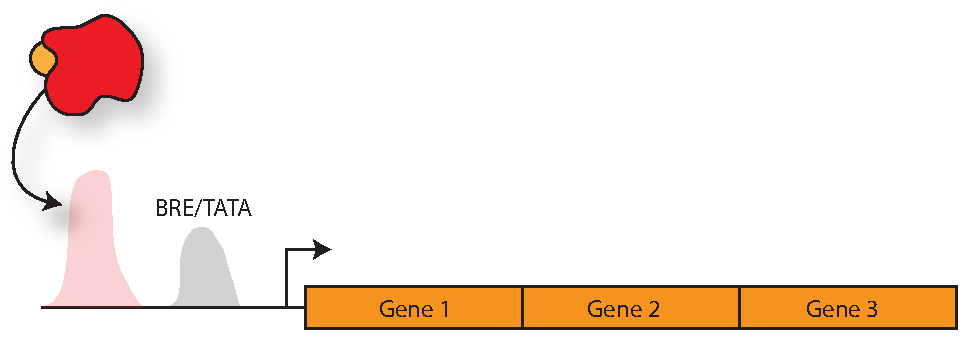
\includegraphics[width=0.9\textwidth]{figures/operon}
 	\caption[Operons: multiple genes transcribed as a single polycistronic transcript]{
 	Operons are co-regulatory units wherein multiple genes are transcribed as a single polycistronic transcript. Several genes involved lactose utilization and transport were discovered to be co-transcribed as a single co-regulated unit in 1961 by Jacob and Monod \cite{jacob_genetic_1961}
}
    \label{fig:chap1:operon}
\end{figure}


\subsubsection{Regulon}

The term \textit{regulon} was coined in 1964 to describe regulation of arginine biosynthetic genes by the repressor, ArgR \cite{maas_studies_1964}. Unlike operons, genes regulated by ArgR are located throughout the genome, including multiple operons like the arginine uptake system, \textit{art}, and histidine transport genes, \textit{hisJQMP}. A regulon consists of genes regulated by a single, common TF (like ArgR). Like operons, there are many regulons in prokaryotes - one for every TF. \textit{E. coli} has 83 annotated regulons \cite{novichkov_regprecise_2012}. The number of genes in a regulon depends on the TF. Sizes can range from several genes to many hundreds, including operons. Several databases collate information about regulons in prokaryotes \cite{alm_microbesonline_2005,novichkov_regpredict:_2010,novichkov_regprecise_2012}. Notably, \href{http://regprecise.lbl.gov/RegPrecise/}{RegRecise} uses evolutionary conservation to refine regulon predictions across multiple species \cite{novichkov_regprecise_2012}.

\begin{figure}[h!]
    \centering
    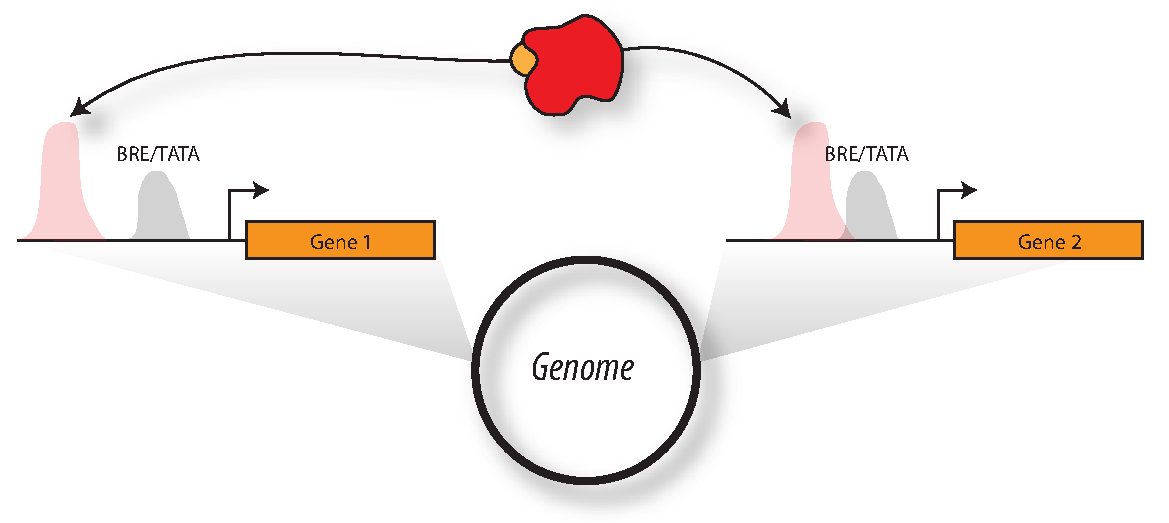
\includegraphics[width=0.9\textwidth]{figures/regulon}
 	\caption[Regulon: multiple gene regulated by a common transcription factor]{
 	A regulon consists of multiple genes or operons located throughout the genome that are co-regulated by a common transcription factor. The ArgR regulon was first described in 1964 by Maas and Clark \cite{maas_studies_1964}.
}
    \label{fig:chap1:regulon}
\end{figure}

\subsubsection{Modulon}

A \textit{modulon} is a collection of operons and regulons that are regulated by a common pleiotropic TF in addition to different specific TFs. Canonical examples include the CAP modulon, a nutrient-responsive modulon that affects the \textit{lac} operon as well as the arabinose catabolism operon (\textit{ara} operon), and the FNR modulon \cite{guest_fnr_1996}, which responds to anaerobiosis. Like regulons, all of the genes of a modulon are regulated by at least one common TF, generally a global regulator (i.e., a TF that regulates many genes, typically on account of its low sequence specificity). 

\subsubsection{Stimulon}

A \textit{stimulon} consists of operons and regulons that are regulated by the same stimulus. Well known examples include the yeast $H_{2}0_{2}$ stimulon \cite{godon_h2o2_1998} and the \textit{B. subtilis} heat shock stimulon \cite{schumann_bacillus_2003}. Stimulons include all of the biological pathways and processes that respond to the same environmental change. As such, they can be large, sometimes including thousands of genes. Stimulon genes can increase as well as decrease in expression.

\subsubsection{Corem}

Co-regulated modules or \textit{corems} are the condition-specific modules discovered by EGRIN 2.0. Unlike other definitions of modular genetic regulation, corems can be regulated by multiple, independent TFs. They can contain subsets of operons and regulons, reflecting condition-specific generation of multiple transcriptional isoforms from an operon. They can include genes from multiple regulons and operons. They range in size from small (3 genes) to large (100s of genes). Corems also vary in how often they are co-expressed, from rare ($<$1/10 of the observations) to common ($>$2/3 of the observations). Importantly, an individual gene can belong to \textit{multiple} corems. A summary of corem statistics for \textit{E. coli} and \textit{H. salinarum} corems is available in Figure \ref{fig:corem_stats}. Defining hallmarks of a corem are depicted in Figure \ref{fig:chap1:corem}. The generation, properties, and utility of corems will be developed throughout the text.

\begin{figure}[h!]
    \centering
    \includegraphics[width=0.6\textwidth]{figures/corem}
 	\caption[Corem: subsets of operons and regulons regulated by multiple transcription factors]{
 	Corems are condition-specific co-regulatory modules discovered by the gene regulatory inference algorithm EGRIN 2.0. Corems can contain subsets of genes from multiple regulons and operons. Each corem has evidence for co-regulation in the form of \textit{cis}-regulatory motifs called gene regulatory elements or GREs. GREs suggest that some corems are regulated by independent factors. Generation and analysis of corems will be described throughout the text. 
}
    \label{fig:chap1:corem}
\end{figure}

\section{Networks in biology}

Networks (or graphs) are mathematical representations of the relationships between objects. Networks consist of nodes (objects) and edges (relationship between the objects). Mathematically, we refer to this entity as a graph, $G = (N,E)$, where the graph, $G$, is an ordered pair comprised of nodes, $N$, and edges, $E$, which themselves are two element subsets of $N$. They can be represented using a (weighted) adjacency matrix, where each entry $N_{i, j}$  indicates a (weighted) relationship between nodes $i$ and $j$.

Networks have become popular to represent biological information, especially from high-throughput screens and experiments. Regulatory influences, protein-protein interaction, and metabolic processes can be represented as networks, where nodes represent regulators, genes, proteins, metabolites or any other biological entity, and edges, which connect nodes, represent arbitrary interactions between the nodes (Figure \ref{fig:chap4:networks}).  A variety of biological networks have been generated, including protein-protein interaction networks \cite{schwikowski_network_2000}, gene regulatory networks  \cite{bonneau_predictive_2007}, metabolic networks  \cite{forster_genome-scale_2003}, even literature citation networks \cite{west_eigenfactor_2010}. Figure \ref{fig:chap4:networks} summarizes important properties of networks. Formalizing biological interactions as networks has a number of analytical advantages. Besides simplifying the representation of biological interactions, graphs have a long, well studied history. Structuring biological relationships in a graph gives access to richly developed tools of graph theory.  Conveniently, many of the mathematical concepts and statistical measures developed for abstract graph structures also apply to biological networks. A graph can be analyzed mathematically to reveal characteristics of its topology. Since the structure of interactions in a network is oftentimes directly related to dynamical properties of that network, topological analysis can give insight into the organization and function of biological systems. Important topological features of biological networks include community structure (e.g., biological modules), hierarchical organization (e.g., nearly power-law degree distributions), and overrepresented network motifs (e.g., the three gene feed-forward loop). These topological features of biological networks and their consequence for the function of biological systems will be explained in more detail throughout the text. 

\begin{figure}[h!]
    \centering
    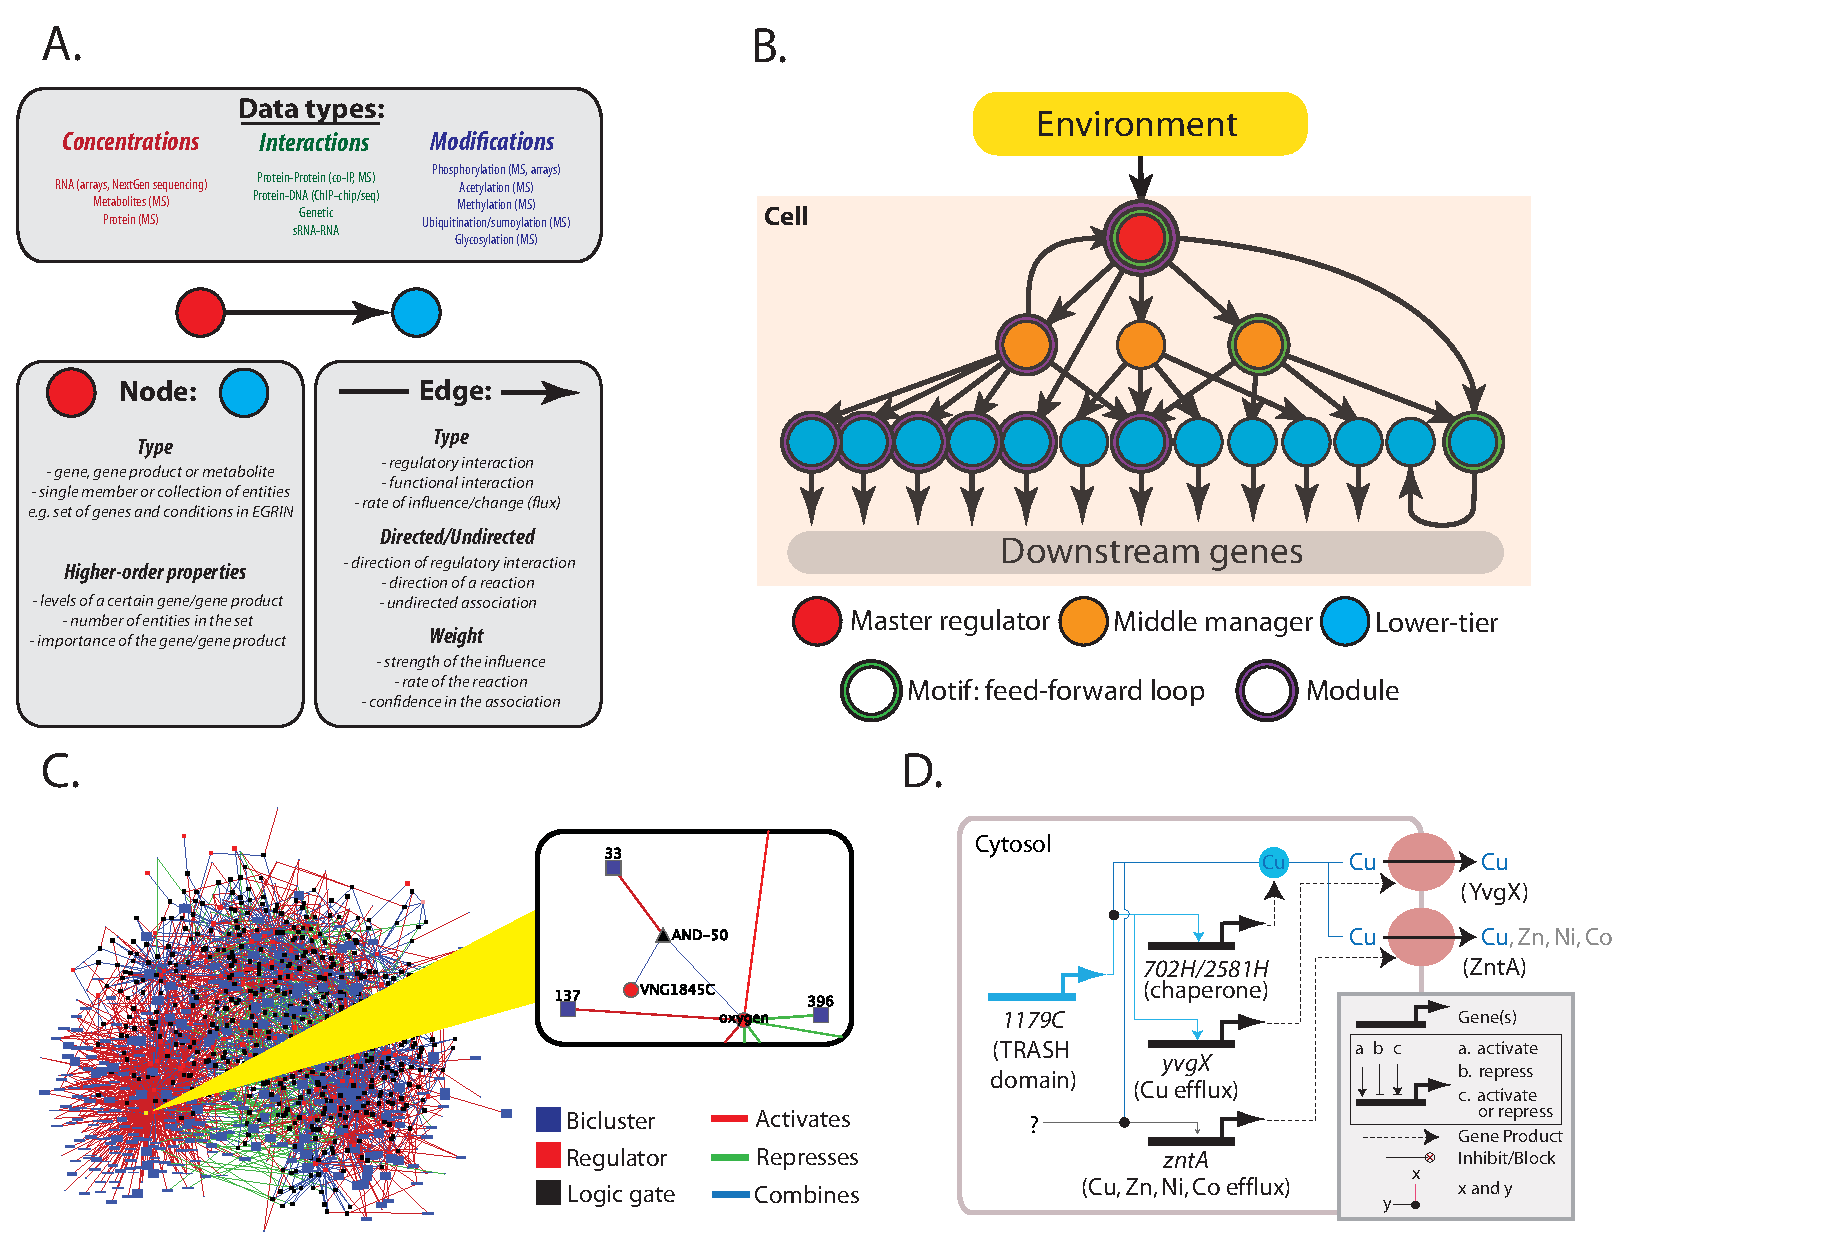
\includegraphics[width=0.9\textwidth]{figures/review_figure1}
 	\caption[Generation and properties of networks]{
 	(A) The fundamental units of a network (or graph) are nodes, and edges. Three types of biological information are commonly represented as a network: transcriptional, metabolic, and protein-protein interactions. (B) Biological networks share common features. (1) hierarchy: transcriptional networks are close to scale-free in the distribution of regulatory connections and exhibit hierarchical arrangement of connections \cite{barabasi_network_2004}. (2) modularity: biological networks aggregate pathways and functions into modules \cite{hartwell_molecular_1999}. Here, we denote a transcriptional “module” by a purple ring surrounding the nodes in the module. (3) motifs: interesting dynamic behaviors of gene circuits are often mediated by particular wiring of the parts, which defines a network motif. The members of a particularly well-studied network motif, the feed-forward loop, are depicted in this illustration by green circles surrounding the nodes \cite{alon_network_2007}. (C) Biological networks learned from experimental data, such as the Environmental and Gene Regulatory Influence Network (EGRIN) for \textit{H. salinarum sp. NRC-1}, contain many layers of information that can be mined to aid hypothesis generation \cite{bonneau_predictive_2007}.
}
    \label{fig:chap4:networks}
\end{figure}

\subsection{Gene regulatory networks (GRNs)}

Regulatory interactions can be cataloged, visualized, and analyzed as gene regulatory networks (GRNs). GRNs can encode who regulates whom, when, where, and to what extent. Analysis of GRNs has revealed valuable insight into how cells process information \cite{barabasi_network_2004} and control expression of their genomes. 

GRN sub-networks that respond to environmental change range from simple to complex. In the simplest case, two-component relay systems directly couple environmental sensing to gene regulation through activation of a TF (e.g., osmoregulation by EnvZ/OmpR two-component system in \textit{E. coli} \cite{aiba_evidence_1989}). Most natural environments, however, change in more complicated ways. Microbes must decipher  many overlapping signals, some of which are prone to high levels of noise. To make the task even more complicated, genetic circuits are not isolated from one another. Even simple relay systems exhibit cross-regulation with other regulatory circuits and can affect other cellular components indirectly \cite{laub_specificity_2007}. To achieve robust response to complicated environmental signals, cells have evolved mechanisms to handle errors, cross-talk, and noise. This accomplished, in part, by encoding gene regulation in combinatorial, modular regulatory circuits that confer robustness to the system.   

\subsection{Discovery and Inference of GRNs}

Obtaining accurate information about regulatory interactions is critical to draw conclusions about biological function from network structure. Considerable effort over the past decade has been dedicated to obtaining accurate GRNs. These efforts fall into two major categories: experimental and computational approaches. The two are not mutually exclusive; in fact, computational approaches always build from experimental observations. The two approaches do, however, vary in the amount of time and money required to obtain comprehensive and accurate GRNs. 

\subsubsection{Experimental Approaches}

Experimental data is the starting point for all GRN reconstruction. An annotated genome is a minimum requirement. The units of the GRN - in this case genes - must be defined. Regulatory proteins (TFs) must also be defined. For newly sequenced genomes, this is accomplished by searching within the new genome for DNA binding domain (DBD) homologies (described above, \ref{pssms}) \cite{bonneau_comprehensive_2004}. Those genes with DBDs are considered putative TFs. 

After basic genome annotation, several approaches for GRN reconstruction exist. The most obvious involves direct measurement of TF binding events across the genome using ChIP-chip or ChIP-seq. Each binding event in the promoter region of a gene (observed after filtering at some confidence threshold) can be considered an edge between a TF and gene in the GRN. Other experimental methods, like \textit{in vitro} binding of purified TF to a promoter  sequence can be used to support the assignment. While attractive, such approaches suffer from two complications: (1) they require separate experiments for each TF. This, in turn, requires developing a purification strategy for each TF, typically using genetic modification (e.g., HA-tag). For bacterial genomes, this would require at least 100 separate strains and experiments for a complete GRN. (2) More troubling, is that observed TF$\rightarrow$gene binding is condition-specific. This means that experimentally-based GRNs only reflect the conditions in which the data were collected. For interaction-based assays (like ChIP-chip or ChIP-seq) to be comprehensive, they would need to be measured in many conditions. Designing experiments to test all pairs of TF and relevant conditions would lead to combinatorial explosion. New technologies like DNase I hypersensitivity \cite{crawford_identifying_2004} promise to overcome some of these challenges by measuring all bound sites throughout the genome in a single experiment. Currently, however, it is difficult to resolve which TF is bound to a particular fragment without \textit{a priori} knowledge of the binding preferences of TFs. Other challenges exist for using these methods in bacterial genomes. 

Several resources have been developed to share experimental knowledge of GRNs across laboratories. RegulonDB, for example, is a database of all evidence for transcriptional regulation collated for \textit{E. coli} \cite{salgado_regulondb_2006}. The collection of data in RegulonDB represents over 50 years of experimental work to characterize the GRN from a single organism. This highlights how challenging it is to reconstruct GRNs directly from experimental data. In the absence of technological innovation, GRN reconstruction in newly sequenced species through experimental approaches alone will be time and cost prohibitive. Many investigators, therefore, have considered alternative approaches to rapidly infer GRNs, especially for understudied organisms. Usually these alternatives employ computational inference methods. 

\subsubsection{Computational Approaches}

Computational approaches attempt to reverse engineer GRNs directly from experimental data. While such methods are always underpowered (i.e., there are too few observations for the number of variables in the system), computational inference methods have made significant improvements, greatly increasing predictive accuracy. One of the biggest gains for these methods came from including biological priors (i.e., using biological knowledge to assist inference). Especially in understudied organisms, computational inference is the only viable alternative to costly, brute force experimentation for GRN reconstruction. 

The primary source of data used for most computational approaches is gene expression. Microarray and RNA-seq allow for quantitation (absolute or relative) of every gene in the genome with a single experiment. To deduce a GRN from these measurements, inference algorithms universally assume that these expression patterns result from some reproducible genetic ``program''. The aim of computational methods is to use data to figure out the program. From this perspective, biological inference is also a problem of pattern recognition (constrained by biological mechanism). Given a sufficient number of observed expression profiles (e.g., different experimental conditions), one can deduce an underlying network that produced them (at least one of many networks that is consistent with the data). The promise of these approaches is that gene expression data is relatively easy and cheap to collect, even in understudied organisms. 

 Full description of computational methods used to infer gene regulatory networks will be provided in Chapter \ref{chap:2} It should be noted that GRN inference methods vary substantially: from correlation to causal, and from statistical to information-based. De Smet \textit{et al.} provide a comprehensive review of GRN inference methods, highlighting the advantages and shortcomings of each \cite{de_smet_advantages_2010}. 

\section{Systems-level view of gene regulatory organization}

 GRN analysis reveals valuable insight into how cells process information. A systems perspective is essential for deciphering how microbes coordinated expression of their genomes. Just as genes work in concert to mediate environmental responses, multiple TFs work together to coordinate the dynamic activity of GRNs. GRNs are impossible to characterize from the perspective of a single TF. 

 Early topological investigations of GRNs revealed several insights. First, not all regulators are equivalent; few transcription factors (TFs) regulate many genes, whereas the majority of TFs regulate far fewer downstream genes (Reviewed in \cite{barabasi_network_2004}). Second, GRNs are hierarchical. ``Master regulator'' TFs, for example, initiate regulatory cascades. While a ``master regulator'' many only interact with few TFs, it can initiate a regulatory cascade by influencing activities of ``middle managers'' that propagate its signal to ``lower tier'' regulators, directly controlling specific processes  \cite{yu_genomic_2006}. Third, some patterns of interactions are statistically overrepresented in biological networks -- these overrepresented subgraphs are called motifs (\cite{milo_network_2002}, Reviewed in \cite{alon_network_2007}). Below I elaborate on the dynamical properties of these features. Finally, abstract representations of gene regulation can yield meaningful dynamic insight into biological processes. Examining the cell-cycle regulatory network as a Boolean representation, for example, reveals the existence of biological attractor states that contribute to the robustness of the cell cycle \cite{li_yeast_2004}.    

As mentioned previously, interpretation of GRNs depends critically on their accuracy. Without correct annotation of TF$\rightarrow$gene relationships, it is impossible to know which TF-gene pairs, for example, are in feed forward loops or which TFs are ``master regulators''.  Network topology is critical to understand network dynamics. In the following sections, I consider the dynamical properties of GRN topological features. 

\subsection{Network Motifs}

Network motifs are frequently appearing topological relationships in directed GRNs. By cataloging frequencies of three gene motifs in \textit{E. coli}, Uri Alon and his colleagues discovered over representation of certain types of motifs in natural GRNs, including feedforward and feedback architectures \cite{milo_network_2002}. These regulatory motifs possess interesting dynamic behaviors, which help cells adjust to changes in their environment. Feedforward loops, for example, buffer noise in highly deterministic biological processes, such as in development \cite{mangan_structure_2003,levine_gene_2005}, while feedback loops provide local sensing and specific response to chemical changes, such as product inhibition exerted in metabolic pathways \cite{neidhardt_escherichia_1996}. Figure \ref{fig:chap1:ffl} provides a graphical representation of the dynamic properties of the feedforward loop. While complete enumeration of all possible three gene architectures made the study by Alon and colleagues possible \cite{milo_network_2002}, there are likely important higher-order motifs in biological systems as well, including global motifs consisting of many component sub-motifs (i.e., motifs of motifs, etc), that may be difficult to assess statistically because of exponential increase in possible topological permutations.

\begin{figure}[h!]
    \centering
    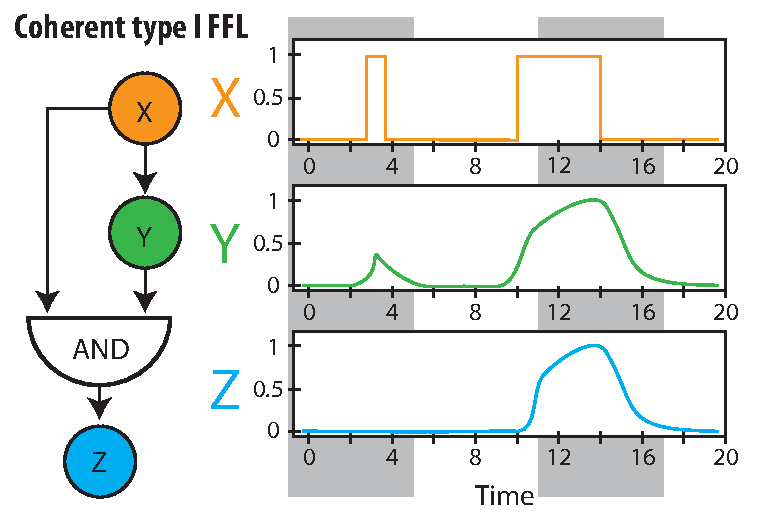
\includegraphics[width=0.7\textwidth]{figures/ffl}
    \caption[Network motifs: the coherent feed-forward loop]{
    The coherent feed-forward motif is a well studied network motif that occurs commonly in biological networks. Like other network motifs, the arrangement of genes into a coherent feed-forward loop has interesting dynamical properties. Feed-forward loops have been shown to buffer noise in biological systems, as well as confer rapid response once a critical signal threshold is reached \cite{mangan_structure_2003}. The cartoon representation depicts downstream expression of $Z$ in response to either a transient or sustained pulse of $X$ (adapted from \cite{mangan_structure_2003}).
}
    \label{fig:chap1:ffl}
\end{figure}

\subsection{Regulatory Logic}

The complete set of TF$\rightarrow$gene interactions in the cell composes a complex regulatory network. This network sets upper and lower bounds on possible expression levels for genes. Dynamic execution of the network leads to coordinated expression of the genome that has evolved to match the sensed environment. Interaction topologies that make up GRNs range in complexity from simple single input motifs (e.g., SIM), to more complicated three gene motifs (e.g., feed forward loop, above), to higher-order architectures involving multiple genes and composed of multiple three-gene (and larger) component motifs (e.g., integrated feedforward loop). These interactions can even compute logic functions, like \textit{and}/\textit{or} gates. Figure \ref{fig:chap1:regLogic} highlights the range of complexity in regulatory logic.

From the standpoint of systems biology, this topological framework helps us understand which genes and functional processes are coordinated in which environments. Observationally, the output of these complex regulatory circuits are co-expression patterns observed in gene expression data. The goal of this project was to group these co-expression patterns into biologically meaningful modules, determine what TFs and regulatory logics were responsible for their generation, and to understand when and why they are co-expressed.  

\begin{figure}[h!]
    \centering
    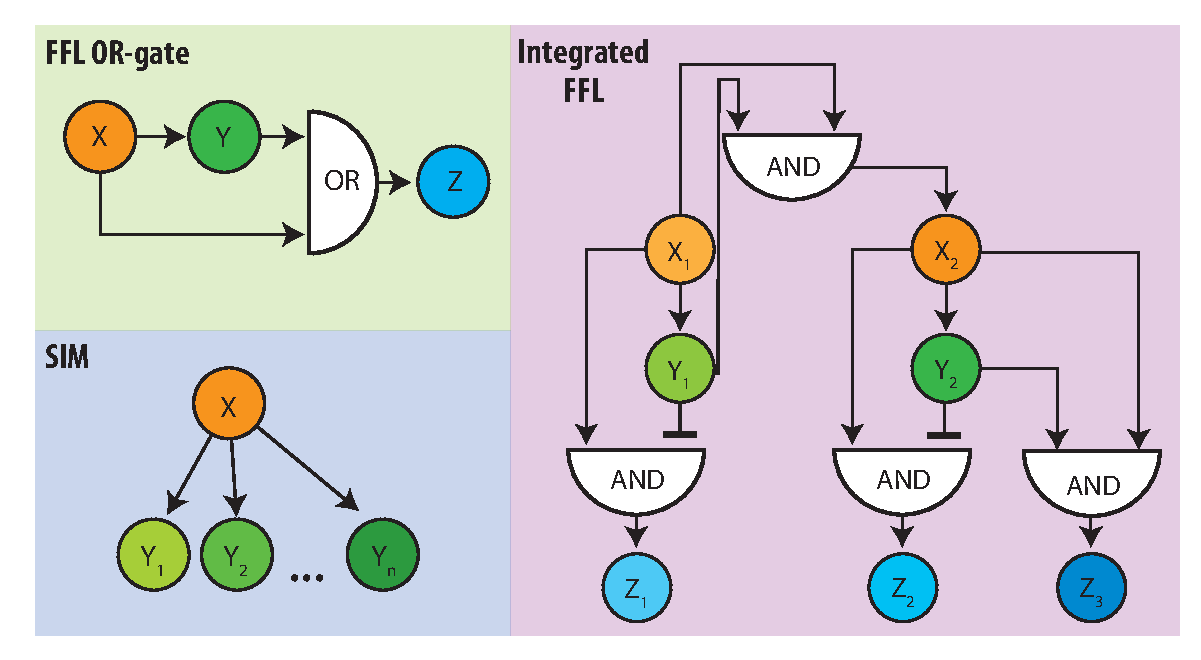
\includegraphics[width=0.9\textwidth]{figures/regLogic}
 	\caption[Varieties of regulatory logic, from simple to complex]{Gene regulatory logic ranges from simple to complex. Three gene regulatory circuits highlight varying degrees of complexity. Note the use of logic gates using \textit{and}/\textit{or} gates. Ultimately, all regulatory sub-circuits (even the simple SIM) are embedded in much more complicated regulatory networks.  
}
    \label{fig:chap1:regLogic}
\end{figure}

\subsection{Beyond the operon and regulon}

In the 1996 edition of \textit{EcoSal}, Neidhardt and Savageau wrote a chapter about regulation of multigene systems entitled, ``Regulation Beyond the Operon'' \cite{neidhardt_escherichia_1996}. The chapter explored concepts of gene expression beyond simple co-linear arrangement of genes in an operon, starting with the regulon and moving to more complex relationships described by modulons and stimulons (described above). While it was clear from the data that genes were co-expressed in complex, condition-specific arrangements, it has been less clear how these patterns emerge from GRN activity. Unresolved questions included: Do genes have to be regulated by a common factor to be consistently co-expressed across environments? What is the role of combinatorial regulation in prokaryotes? Are genes regulated by a common factor always co-expressed? This project attempts to quantify the relationship between gene regulatory modules, GRNs, and the nuanced condition-specific associations between TFs and genes that generate condition-specific co-regulatory modules - directly from data. 

\section{Chapter Organization}

The following chapters investigate the organization, function, and evolution of GRNs in prokaryotes. I develop a comprehensive view of data-driven GRN inference, from model construction (Chapter \ref{chap:2}) to interpretation (Chapter \ref{chap:3}) and implications (Chapter \ref{chap:5}). I explore how the structure and function of GRNs contributes to our understanding of how these networks evolve (Chapter \ref{chap:4}) . 

Chapter \ref{chap:2} discusses computational methods for gene regulatory network inference from genome sequence and large gene expression compendiums. It also describes construction of \egrine, the network ensemble elaborated throughout the text. In addition to complete description of the algorithm, many additional details are documented, including experimental data sets used, benchmarks employed to evaluate model performance, and web-framework developed to facilitate exploration of the model's predictions. Chapter \ref{chap:3} focuses on biological interpretation of \egrine. In particular, it documents the model-assisted discovery of \textit{corems}, condition-specific co-regulatory modules that influence cellular fitness. \ref{chap:4} shifts focus to the evolution of GRNs. I consider how dynamics of environmental change shapes the way GRNs evolve. Finally, \ref{chap:5} investigates the consequences and suggests directions forward, both for improving GRN inference and in context of evolution. 


 

 
 